% Copyright 2007 by Till Tantau
%
% This file may be distributed and/or modified
%
% 1. under the LaTeX Project Public License and/or
% 2. under the GNU Public License.
%
% See the file doc/licenses/LICENSE for more details.



\documentclass{beamer}

%
% DO NOT USE THIS FILE AS A TEMPLATE FOR YOUR OWN TALKS�!!
%
% Use a file in the directory solutions instead.
% They are much better suited.
%


% Setup appearance:

\usetheme{Bergen}
\usefonttheme{professionalfonts}
\usecolortheme{default}

\setbeamertemplate{navigation symbols}{}


% Standard packages

\usepackage[english]{babel}
\usepackage[latin1]{inputenc}
\usepackage{times}
\usepackage[T1]{fontenc}
\usepackage{graphicx}

% Setup TikZ

\usepackage{tikz}
\usetikzlibrary{arrows}
\tikzstyle{block}=[draw opacity=0.7,line width=1.4cm]


% Author, Title, etc.

\title
{%
  A Handful of Numerical Integration
}

\author
{
 Minqi~Pan
}

\institute
{
Capital Normal University
}

\date{\today}


% The main document

\begin{document}

\begin{frame}
  \titlepage
\end{frame}

\frame
{
  \frametitle{The Thing about Numerical Integration is ...}
  
  \begin{itemize}
  \item<1->   ... to find algorithms for calculating the numerical value of a definite integral.
  \item<2-> ... a.k.a. numerical quadrature (often abbreviated to quadrature) 
  \item<3-> ... oh, that's only for one-dimensional 
  \item<4-> ... `cubature` for Numerical integration over more than one dimension
  \end{itemize}
}


\begin{frame}[t]{So the problem is}
  \begin{block}{Inputs}
  a definite integral:
   \[ S=\int_a^b\! f(x)\, dx. \]
  \end{block}
  \begin{block}{Output}
an approximate solution of it!
  \end{block}
    \begin{block}{Actually}
    
    \begin{itemize}
    \item <1->
    continuous functions have exact analytical solutions.
\[
    \int_a^b\! f(x)\, dx = F(b) - F(a). \]
        \item<2->\alert{Yet no one cases about it!}
    \end{itemize}
\end{block}
\end{frame}

\begin{frame}{Why we do NOT care \dots}
  \begin{enumerate}
  \item<1-> \alert{Data may be sampled.}
    \begin{itemize}
    \item<2-> in which case \dots
    \item<3-> The integrand $f(x)$ is known only at certain points
    \item<4-> embedded systems and other computer applications
    \end{itemize}
  \item<5-> \alert{No perfect students can find all antiderivatives.}
    \begin{itemize}
    \item<6-> Even though it's an elementary function
    \item<7-> Some say it's impossible.
    \item<8-> Remember this? \[f(x) = e^{-x^2}\]
    \item<9-> Know this?Gauss error function \[    \operatorname{erf}(x) = \frac{2}{\sqrt{\pi}}\int_{0}^x e^{-t^2} dt. \]
   	that's his antiderivative! (constant-timing-wise)
    \item<10-> Know this? "Gauss error function" \[    \operatorname{erf}(x) = \frac{2}{\sqrt{\pi}}\int_{0}^x e^{-t^2} dt. \]
   	that's his antiderivative! (constant-timing-wise)
	  \item<11-> can it be written in elementary form?
    \end{itemize}
  \end{enumerate}
\end{frame}


\begin{frame}{when they CAN'T they CHEAT}
when the day is too dark for antiderivatives, they \dots
  \begin{enumerate}
  \item<1-> give answers as an infinite series or product
  \item<2->  mess answers with special functions
  \item<3->  that's what we call symbolically
  \end{enumerate}
\end{frame}



\begin{frame}{So try the other flavor}
Now begins the days of Numericallarity.

\end{frame}



\begin{frame}{It has a history!}

\includegraphics{pythagoras}\\
Mathematicians of Ancient Greece, according to the Pythagorean doctrine, understood calculation of area as the process of constructing geometrically a square having the same area (squaring). 
\end{frame}
\begin{frame}{It has a history!}
cyclotomic method by ancient Chinese Mathematician Liu Heng\\
    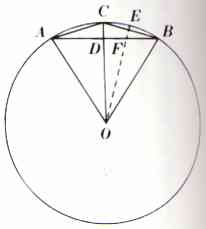
\includegraphics{774855368773189da2cc2b39}
\end{frame}

\begin{frame}{It has a history!}
    
\includegraphics{4d4970065e79c227030881ee}
\end{frame}




\begin{frame}{Basic Approach}
\huge{
integrand $\rightarrow$ integral}
\end{frame}


\begin{frame}{Basic Approach}
So, 
{\huge
integrand $\rightarrow$ integral}
  \begin{enumerate}
  \item<1->  we do it finitely
  \item<2->  combine the evaluations of the integrand
  \item<3->  that is, weighted sum of these values
  \item<4->  get an approximation to the integral

  \end{enumerate}


\end{frame}

Quadrature


\begin{frame}{Good/Bad Messures}
And, {\huge
error}
  \begin{enumerate}
  \item<1->  is unavoidable
  \item<2->  We want to know the number of integrand evaluations
  \item<3->  result in what approximation errors?
  \item<4->  small number of evaluations $\Rightarrow$ small error is good

  \end{enumerate}


\end{frame}


\begin{frame}{rectangular rule}
\[    \int_a^b f(x)\,dx \approx (b-a) \, f\left(\frac{a+b}{2}\right). \]
    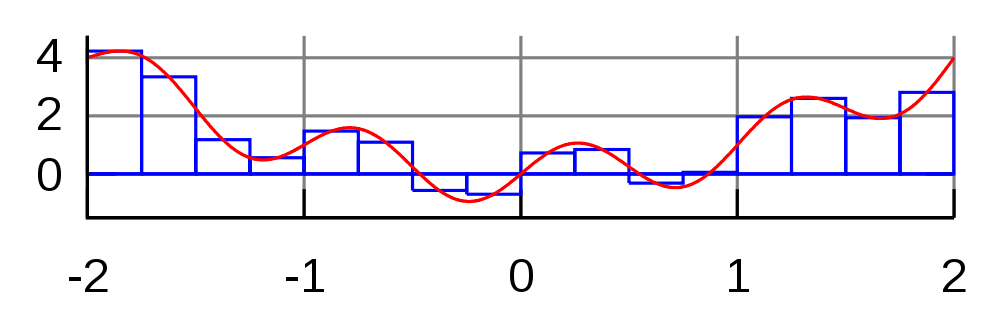
\includegraphics[width=\textwidth]{rectangle}

\end{frame}


\begin{frame}{trapezoidal rule}
\[    \int_a^b f(x)\,dx \approx (b-a) \, \frac{f(a) + f(b)}{2}. \]
    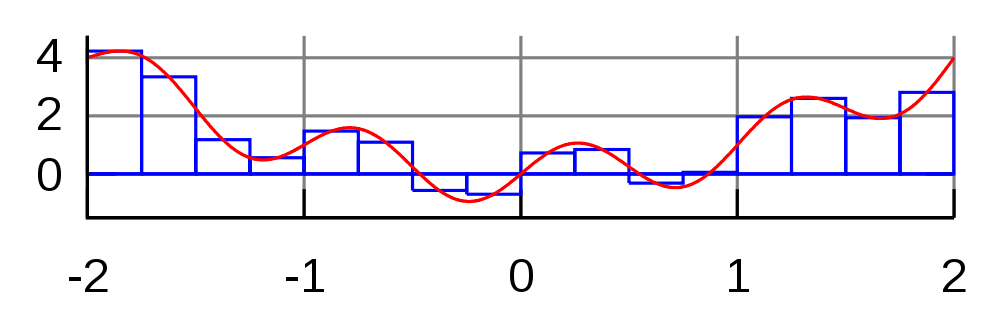
\includegraphics[width=\textwidth]{rectangle}
\end{frame}


\begin{frame}{Simpson's rule}\[    \int_a^b f(x)\,dx \approx \]\[ \frac{b-a}{n} \left( {f(a) + f(b) \over 2} + \sum_{k=1}^{n-1} f \left( a+k \frac{b-a}{n} \right) \right) \]

    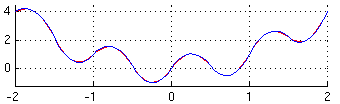
\includegraphics[width=\textwidth]{Integration_simpson}

\end{frame}

\begin{frame}{Adaptive quadrature}

If $f(x)$ does not have many derivatives at all points, or if the derivatives become large, then Gaussian quadrature is often insufficient. In this case, an algorithm similar to the following will perform better:

\end{frame}


\begin{frame}{ Extrapolation methods}

The accuracy of a quadrature rule of the Newton-Cotes type is generally a function of the number of evaluation points. The result is usually more accurate as number of evaluation points increases, or, equivalently, as the width of the step size between the points decreases. It is natural to ask what the result would be if the step size were allowed to approach zero. This can be answered by extrapolating the result from two or more nonzero step sizes, using series acceleration methods such as Richardson extrapolation. The extrapolation function may be a polynomial or rational function. Extrapolation methods are described in more detail by Stoer and Bulirsch (Section 3.4) and are implemented in many of the routines in the QUADPACK library.

\end{frame}



\begin{frame}{ error estimation}
Let f have a bounded first derivative over [a,b]. The mean value theorem for f, where x < b, gives

\[    (x - a) f'(y_x) = f(x) - f(a)\]
for some yx in [a,x] depending on x. If we integrate in x from a to b on both sides and take the absolute values, we obtain

  \[  \left| \int_a^b f(x)\,dx - (b - a) f(a) \right| = \]\[\left| \int_a^b (x - a) f'(y_x)\, dx \right| \]
\end{frame}

\begin{frame}{Truncation error}
Trunction errors in numerical integration are of two kinds:

    local truncation errors � the error caused by one iteration, and
    global truncation errors � the cumulative error cause by many iterations.

\end{frame}


\begin{frame}{Integrals over infinite intervals}
One way to calculate an integral over infinite interval,
\[    \int_{-\infty}^{+\infty}f(x) \, dx, \]
is to transform it into an integral over a finite interval by any one of several possible changes of variables, for example:
\[    \int_{-\infty}^{+\infty} f(x) \, dx = \int_{-1}^{+1} f\left( \frac{t}{1-t^2} \right) \frac{1+t^2}{(1-t^2)^2} \, dt, \]
The integral over finite interval can then be evaluated by ordinary integration methods.
\end{frame}


\begin{frame}{Multidimensional}
The quadrature rules discussed so far are all designed to compute one-dimensional integrals. To compute integrals in multiple dimensions, one approach is to phrase the multiple integral as repeated one-dimensional integrals by appealing to Fubini's theorem. This approach requires the function evaluations to grow exponentially as the number of dimensions increases. Two methods are known to overcome this so-called curse of dimensionality.
\end{frame}

\begin{frame}{Sparse grids}
Sparse grids were originally developed by Smolyak for the quadrature of high dimensional functions. The method is always based on a one dimensional quadrature rule, but performs a more sophisticated combination of univariate results.
\end{frame}



\begin{frame}{Half-infinite intervals}
Monte Carlo methods and quasi-Monte Carlo methods are easy to apply to multi-dimensional integrals, and may yield greater accuracy for the same number of function evaluations than repeated integrations using one-dimensional methods.

A large class of useful Monte Carlo methods are the so-called Markov chain Monte Carlo algorithms, which include the Metropolis-Hastings algorithm and Gibbs sampling.
\end{frame}

\end{document}








